\chapter{Implementation}\label{ch:implementation}

\section{Data Mining} \label{sec:DataMining}
\subsubsection{Data Set}
Any neural network requires data in order to learn and become useful. As such, the training data is an important part of the learning process. For this implementation, the OpenSLR LibriSpeech ASR corpus was imported to provide training data.\\\\
The LibriSpeech is comprised of approximately 1000 hours of 16kHz English read speech in .flac format, and was prepared by Vassil Panayotov with the assistance of Daniel Povey. It is based on audio books from the LibriVox project that have been segmented and aligned. It contains 3 different sets, differentiated by type and size.\\\\
The first, and smallest one, is made of 6.3 GB of "clean" speech, representing approx. 100 hours. "Clean" speech refers to audio recordings where noise and disturbances that might corrupt their quality were eliminated as much as possible.
The second set is made of 23 GB of "clean" speech that represents approx. 360 hours.\\\\
Any neural network requires data in order to learn and become useful. As such, the training data is an important part of the learning process. For this implementation, the OpenSLR LibriSpeech ASR corpus was imported to provide training data.
The LibriSpeech set is comprised of approximately 1000 hours of 16kHz English read speech in .flac format, and was prepared by Vassil Panayotov with the assistance of Daniel Povey. It is based on audio books from the LibriVox project that have been segmented and aligned. It contains 3 different sets, differentiated by type and size.\\\\
The first, and smallest one, is made of 6.3 GB of "clean" speech, representing approx. 100 hours. "Clean" speech refers to audio recordings where noise and disturbances that might corrupt their quality were eliminated as much as possible.
The second set is made of 23 GB of "clean" speech that represents approx. 360 hours.
The final set is made of 30 GB of "other" speech, representing approx. 500 hours of audio. "Other" speech refers to recordings that contain a certain degree of audio disturbance.
The corpus also contains smaller sets for validation and testing.

\subsubsection{Data processing}
As presented above, the OpenSLR corpus provides many features for training neural networks. It is especially efficient for speech recognition systems. However, the current implementation was designed to use pairs of .wav and .txt files as input. Each .wav file represents the audio information that is encoded in the corresponding .txt file, more specifically short paragraphs.\\\\
As presented above, the OpenSLR corpus provides many features for training neural networks. It is especially efficient for speech recognition systems. However, the current implementation was designed to use pairs of \textbf{.wav} files and \textbf{.txt} files as input. Each \textbf{.wav} file represents the audio information that is encoded into the corresponding \textbf{.txt} file, more specifically short paragraphs.\\\\
Unfortunately, this data set is prepared in a different format. There is a single \textbf{.txt} file that corresponds to many \textbf{.wav} files and these are organized in bigger sets. Because of this, the data in its original form is not usable for the current neural network. To prepare the data, certain scripts were implemented in Python.\\\\
The first algorithm is designed to navigate a folder path and its sub-folders to convert all \textbf{.flac} files to \textbf{.wav}. It uses the os and pydub libraries. 
To access every sub-folder in the path, os.walk is used. This function returns the root folder and a list of files and directories in root, after which an internal folder becomes the new root\\
\lstinputlisting[language=Python, flexiblecolumns=true, caption=Folder navigator. , firstline=37, lastline=51]{code/FlacToWavPy.py}

The conversion is handled by another function that uses the pydub library to load the .flac, parse the name and   export the converted .wav file.

\lstinputlisting[language=Python, flexiblecolumns=true, caption=Flac to wav conversion. , firstline=25, lastline=35]{code/FlacToWavPy.py}

The second algorithm navigates the folders in the same way, by using the os.walk method. Then it checks for .txt files by parsing their name. 

\lstinputlisting[language=Python, flexiblecolumns=true, caption=Text file check. , firstline=13, lastline=22]{code/txtFileMaker.py}

The format of the text files in this audio set is known. Using this information, the file name and content is parsed, creating new text files for every paragraph that corresponds to a flac file. This is achieved by exploiting the file name in relation to the beginning and end of each paragraph inside the file.
 
\lstinputlisting[language=Python, flexiblecolumns=true, caption=Text file parsing. , firstline=36, lastline=51]{code/txtFileMaker.py} 
 
\section{DSR System Implementation}

The complete DSR system is the sum of all the previously described parts. Firstly, a recurrent neural network model was designed and implemented. Following, the model was trained on the available data.
Afterwards, the distributed part was focused on. The VPN was set up, and the client-server architecture took form using Python based, TCP sockets.\\\\
Normal operation for the system is as follows:
\begin{enumerate}
\item The server is initialized
\item The client connects to the server
\item The client sends an audio file
\item The server decodes the audio into text
\item The server sends the text to the client
\end{enumerate}
The file sent by the client can be either a microphone recording stored as a .wav at run-time, or an existing .wav file. To store this file, the server expects to receive multiple chunks of a fixed byte size from the client, shown below:
\lstinputlisting[language=Python, flexiblecolumns=true, caption=Server receiving file, firstline=30, lastline=35]{code/serverPy.py} 
After a successful transfer, the server forks a new process. 
This new process runs a script that loads the trained neural network and decodes the received audio file. A pipe is opened between the two processes for the decoded text to be sent back to the client.

\lstinputlisting[language=Python, flexiblecolumns=true, caption=New process, firstline=39, lastline=40]{code/serverPy.py}
The result is received by the client and displayed on screen.

\section{Testing}


The original speech sent to the server was: "he began a confused complaint against the wizard who had vanished behind the curtain on the left".

\begin{figure}[H]
	\centering
	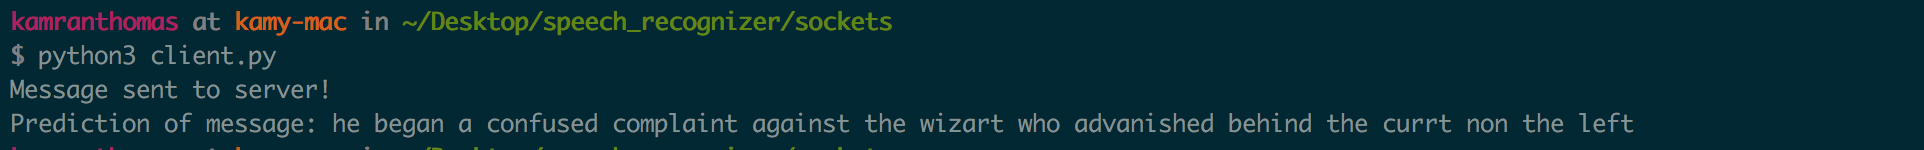
\includegraphics[width=\textwidth]		
	{implementation/client_server_conn}
	\caption{Client side sending message and recieving prediction from server side.}
	\label{fig:client_server_conn}
\end{figure}






